\documentclass[journal]{IEEEtran}

%\documentclass{article}
\usepackage[utf8]{inputenc}
\usepackage{amsmath,amsthm,amssymb,amsfonts, enumerate, graphicx, hyperref}

\title{Proposed Design Project for Phot1x}
\date{January 2021}
\author{christopher\_phenicie}

\begin{document}

\maketitle

\section{Introduction}
\label{sec:intro}

The proposed chip will contain a total of seven interferometers, providing data for two different tests. The first test is understanding the relationship between the free spectral range (FSR) of a Mach-Zehnder interferometer (MZI) as the difference in lengths of the two legs is changed, which will allow for a careful measurement of the group index of the waveguides used in the MZI. The second test is looking at the repeatability of the waveguides by looking at two nominally identical Michelson interferometers with a large ($\sim$~1mm) path length difference. These interferometers will be sensitive to small changes in the group index due to fabrication imperfections, and we can bound the fabrication imperfections based on the observed variations in the measured FSR.

\section{Theory}
\label{sec:theory}

The group index of a material can be measured from the FSR of the fringes in an unbalanced interferometer of known length difference $\Delta L$. Let us consider the case of an interferometer composed of lossless Si photonic waveguides. As described in~\cite{Chrostowski2015}, an MZI can be built on a silicon photonic chip using two Y-branches, one as a splitter to split the incoming light between two waveguides of length $L_1$ and $L_2$, and the other Y-branch used as a coupler to allow the light to interfere. We can describe the power measured at the output of the interferometer as follows:

First, the incoming light described by the electric field $E_i$ is split into the two branches of the Y-branch equally, meaning the field into the two waveguides are $E_1 = E_2 = \frac{E_i}{\sqrt{2}}$. These fields are then propagated along the waveguides, which have effective index $n_1$ and $n_2$ and lengths $L_1$ and $L_2$ respectively. Therefore, the fields at the opposite end of the waveguides are $E_{o1} = \frac{E_i}{\sqrt{2}} e^{-i \beta_1 L_1}$ and $E_{o2} = \frac{E_i}{\sqrt{2}} e^{-i \beta_2 L_2}$ where we define the propagation constant 

\begin{equation}
\beta = \frac{2\pi n}{\lambda}
\label{eq:beta}
\end{equation}
where $n$ is the (effective) index of refraction of the waveguide, and $\lambda$ is the wavelength of the light.

The combining Y-branch will then mix these two fields, producing the output field 

\begin{equation}
E_o = \frac{E_{o1} + E_{o2}}{\sqrt{2}} = \frac{E_i}{2} \left(e^{-i \beta_1 L_1} + e^{-i \beta_2 L_2} \right)
\end{equation}

In these experiments, we will only consider the intensity of the output light $I_o = |E_o|^2$, which can be simplified to the final equation which we will refer to as the transfer function of the MZI:

\begin{equation}
I_o/I_i = \frac{1}{2} (1 + \cos{(\beta_1 L_1 - \beta_2 L_2)})
\label{eq:trans_full}
\end{equation}

For now, we will assume that the waveguides are made of identical material, such that $\beta_1 = \beta_2 = \frac{2 \pi n_{\text{eff}}}{\lambda}$ where $n_{\text{eff}}$ is the effective index of the waveguide. Then, defining the difference in the path lengths of the two legs of the interferometer $\Delta L = L_2 - L_1$, we arrive at the following equation for the tranfer function of the imbalanced MZI with waveguides made of identical material:

\begin{equation}
\frac{I_o}{I_i} = \frac{1}{2} \left(1 + \cos{(\beta \Delta_L)}\right) = \frac{1}{2} \left(1 + \cos{\left(\frac{2\pi n_{\text{eff}} \Delta_L}{\lambda}\right)}\right)
\end{equation}

Note that this is a periodic function that varies with the wavelength of the light $\lambda$. So, if we take a spectrum of this device, that is, measure $I_o$ for a range of different wavelengths, we should see a periodic pattern, undergoing one full oscillation between the wavelength $\lambda_1$ and $\lambda_2$ satisfying the relationship 

\begin{equation}
|\beta(\lambda_1) - \beta(\lambda_2)| \Delta L = 2 \pi
\label{eq:FSR_cond}
\end{equation}
where $\beta$ depends on wavelength both from the appearance of $\lambda$ in the denominator of equation \ref{eq:beta}, but also because the index of refraction of materials (especially the effective index of the photonic waveguide) is wavelength dependent.  

We can then approximate equation \ref{eq:FSR_cond} by assuming that the wavelength difference is small enough that we have

\begin{equation}
(\beta(\lambda_1) - \beta(\lambda_2)) \approx \frac{d\beta}{d\lambda} \Delta \lambda
\label{eq:deltabeta}
\end{equation}

Differentiating equation \ref{eq:beta}, we have

\begin{equation}
\frac{d\beta}{d\lambda} = 2\pi\left(\frac{dn}{d\lambda}\frac{1}{\lambda} - \frac{n}{\lambda^2} \right) = - \frac{2\pi  n_g}{\lambda^2}
\label{eq:dbeta}
\end{equation}
where we have used the definition of the group index 

\begin{equation}
n_g = n - \lambda \frac{dn}{d \lambda}
\label{eq:ngdef}
\end{equation}


Plugging equations \ref{eq:deltabeta} and  \ref{eq:dbeta} back into equation \ref{eq:FSR_cond}, we have that the spacing $\Delta \lambda$ corresponding to one full oscillation (the FSR) is 

\begin{equation}
FSR = \frac{\lambda^2}{n_g \Delta L}
\label{eq:FSR}
\end{equation}

So, if we find the peaks of the spectrum around the wavelength of interest and find the average spacing between them, $FSR$, we can solve for the group index using the formula

\begin{equation}
n_g = \frac{\lambda^2}{FSR \times \Delta L}
\label{eq:solveng}
\end{equation}

Thus, we will use equation \ref{eq:solveng} on the spectrum of the first five interferometers and compare this with the models that will be computed in section \ref{sec:model}.

We can then test the variability of this value due to fabrication imperfections. To maximize sensitivity to imperfections, we will use a long path length difference between the two legs, and use a Michelson interferometer (which gives twice the path length difference for the same length imbalance as the MZI). We can compute the variation in the FSR between the different devices to put a bound on the variation in the width of the waveguide. Specifically, we can bound this by assuming all the observed variation is due to width variations. Then, differentiating equations \ref{eq:FSR} with respect to the waveguide width, we find

\begin{equation}
\frac{d(FSR)}{dw} = \frac{-\lambda^2}{\Delta L \, n_g^2} \frac{dn_g}{dw}
\end{equation}
where recall that for a Michelson interferometer $\Delta L$ is twice the length imbalance. The quantity $\frac{dn_g}{dw}$ can be computed in simulation, so that we can arrive at the following equation relating the measured difference in FSR to the implied maximum width variation:

\begin{equation}
\Delta w = - \frac{\Delta (FSR) \times \Delta L \times n_g^2}{\lambda^2 \times \frac{dn_g}{dw}}
\label{eq:dw}
\end{equation}

\section{Modeling and simulation}
\label{sec:model}


The interferometers in the project will be constructed from strip waveguides etched into an SOI chip with a 220 nm thick Si layer and a capping oxide layer. We will choose the waveguides to be 500nm wide and we will work with the TE mode of the waveguide. These structures can be simulated using the finite difference time domain (FDTD) technique. As an example, the spatial distribution of the waveguide mode from this FDTD simulation is shown in figure \ref{fig:mode}

\begin{figure}[t!]
  \centering
  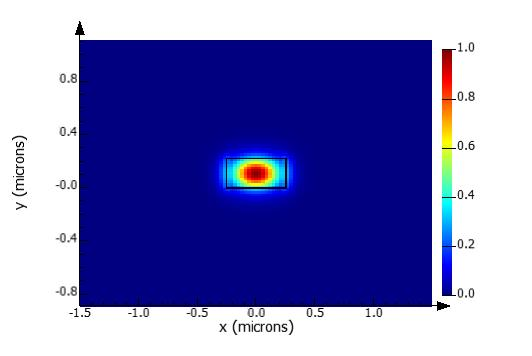
\includegraphics[width = 3.25in]{fig/waveguide_TE.jpg}
  \caption{FDTD simulation of quasi-TE mode of the waveguides we will use in this project, computed using Lumerical MODE. This image is oriented in a plane perpendicular to the direction of light propagation.}
  \label{fig:mode}
\end{figure}

One of the essential parameters needed to predict the properties of the MZI is the index of refraction. More specifically, it is important to have an understanding of the effective index of refraction ($n_{\text{eff}}$) which determines the phase velocity of light in the medium. Additionally, if $n_{\text{eff}}$ is known as a function of wavelength, it can be used to compute the group index of medium ($n_g$), which is ultimately the quantity needed to predict the behavior of the MZI. These parameters can be extracted from the FDTD simulation, as shown in figures \ref{fig:neff} and \ref{fig:ng}. 

\begin{figure}[t!]
  \centering
  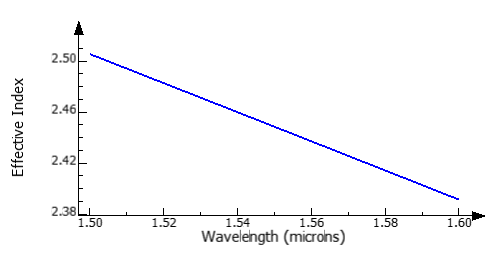
\includegraphics[width = 3.25in]{fig/waveguide_dispersion_narrow.png}
  \caption{Variations in the effective index of the proposed waveguide as a function of wavelength. Values are computed from FDTD simulations in Lumerical MODE.}
  \label{fig:neff}
\end{figure}


\begin{figure}[t!]
  \centering
  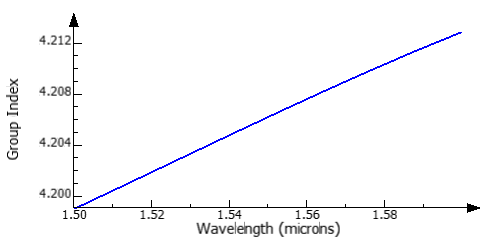
\includegraphics[width = 3.25in]{fig/group_index_narrow.png}
  \caption{Variations in the group index of the proposed waveguide as a function of wavelength. Values are computed from FDTD simulations in Lumerical MODE, and are generally in agreement with the simulated effective index.}
  \label{fig:ng}
\end{figure}

This information can then be distilled into a compact model for this waveguide by fitting the effective index to a low-order polynomial:

\begin{equation}
n(\lambda)\approx a_0 + a_1(\lambda - \lambda_0) + a_2(\lambda - \lambda_0)^2
\end{equation}

Where we arrive at the following fit parameters from the above data:

$ a_0 = 2.4489, a_1 = -1.1337, a_2 = -0.0451 $.

Note that if we use this compact model along with equation \ref{eq:ngdef}, we find good agreement between the simulated and calculated values of the group index.

Armed with this knowledge, we can now simulate the two proposed devices and see how the simulations compare to the predictions from the equations laid out in section \ref{sec:theory}.

The basic MZI circuit will be composed of Y-branches on the input and output, with each leg of the interferometer composed of a strip waveguide of varying length or width, as shown in figure \ref{fig:schematic}.


\begin{figure}[t!]
  \centering
  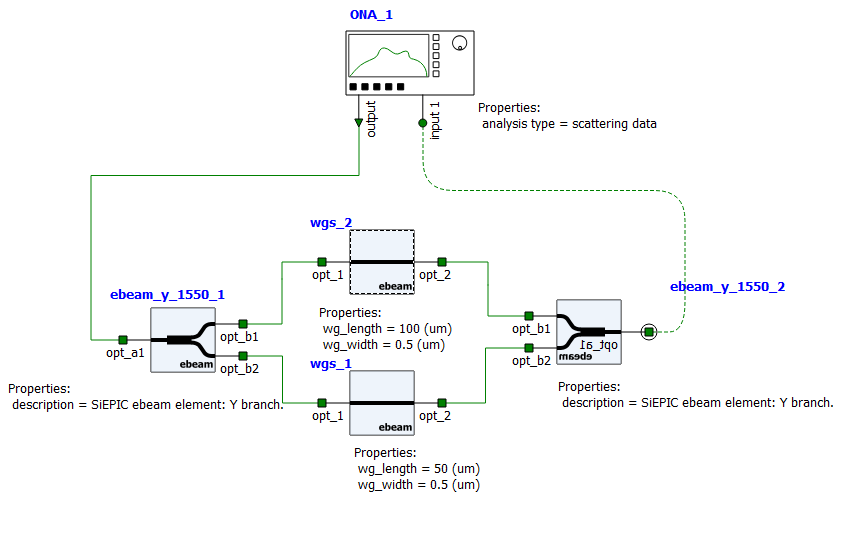
\includegraphics[width = 3.25in]{fig/MZI_schematic.png}
  \caption{Proposed schematic of the MZI. As it is drawn, the top waveguide (labelled ``wgs\_2") is imbalanced in length by 50 $\mu$m compared to the bottom waveguide}
  \label{fig:schematic}
\end{figure}

We can simulate the behavior of this device in Lumerical INTERCONNECT, as shown in figure \ref{fig:deltaL}. We can see the calculated FSR from these simulations are well captured by the transfer function of the MZI (eq \ref{eq:trans_full}) and the predicted FSR computed from it (i.e. eq \ref{eq:FSR}), as shown in table \ref{tab:MZI}.

\begin{figure}[t!]
  \centering
  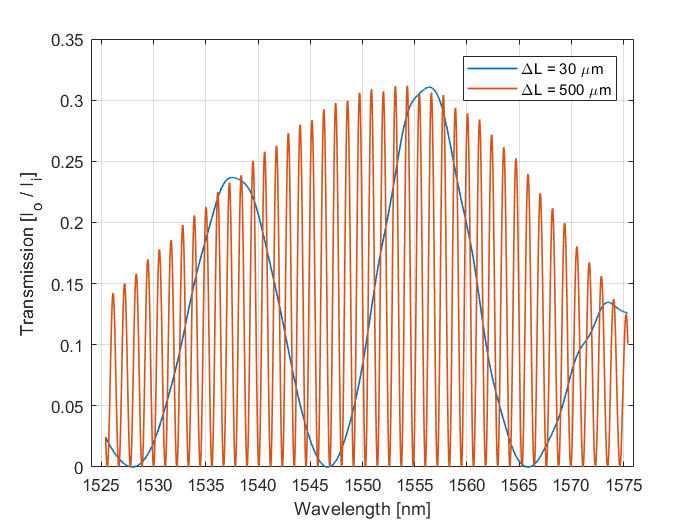
\includegraphics[width = 3.25in]{fig/MZI_length_variation.png}
  \caption{Simulated transfer function of the MZI device shown in figure \ref{fig:schematic} for two different length imbalances in the interferometer. Only two of the transfer functions are shown for clarity, the full data set is summarized in table \ref{tab:MZI}}
  \label{fig:deltaL}
\end{figure}



\begin{table}
\centering
\begin{tabular}{ r | r | r }
  \hline
  $\Delta L (\mu m)$ & Calculated FSR (nm) & Simulated FSR (nm) \\
  \hline
  30                 & 19.040              & 17.995 \\
  50                 & 11.424              & 11.247 \\
  100                & 5.712               & 5.682 \\
  300                & 1.904               & 1.900 \\
  500                & 1.142               & 1.142 \\
\end{tabular}
\caption{Comparison of the FSR calculated from equation \ref{eq:FSR} compared to the value extracted from the simulations in Lumerical INTERCONNECT}
\label{tab:MZI}
\end{table}

The proposed Michelson interferometer is shown in figure \ref{fig:mich-scheme}, where we have used loop waveguides as mirrors and we are using broadband directional coupler to split the light in order to be able to measure the reflected signal. Note the large length imbalance of the two branches.

\begin{figure}[t!]
  \centering
  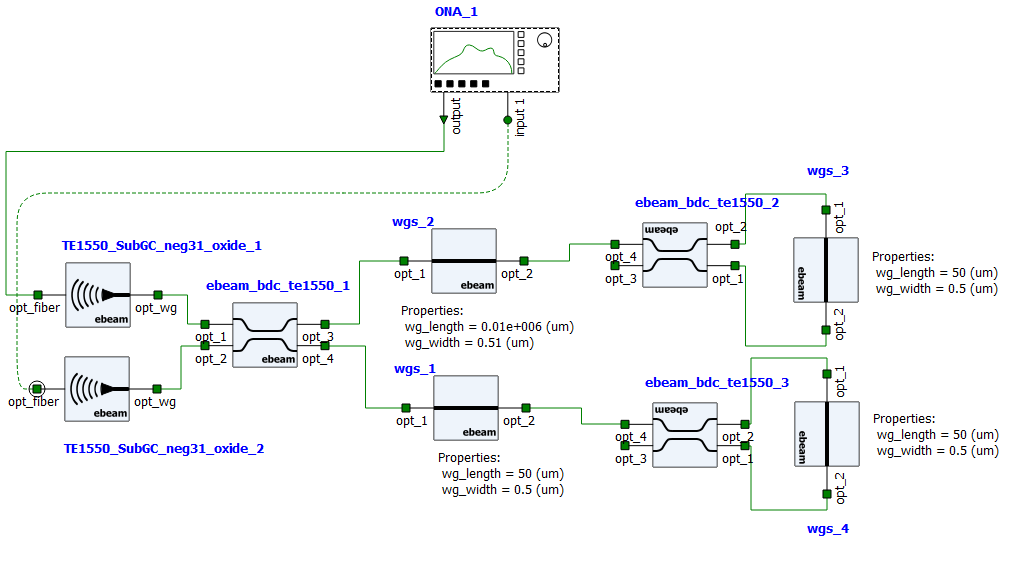
\includegraphics[width = 3.25in]{fig/Michaelson_schematic.png}
  \caption{Schematic of the proposed Michelson interferometer.}
  \label{fig:mich-scheme}
\end{figure}

We can simulate the transfer function of this device in Lumerical INTERCONNECT for waveguides of width 500nm and 510nm. The spectrum contains many oscillations, but we can see that there is a phase shift of $\pi$ between the devices in just a 5nm bandwidth, as shown in figures \ref{fig:mich-in} and \ref{fig:mich-out}. If we compute the change in FSR between the entire 50nm bandwidth of the grating couplers, we should have sensitivity much better than this.

\begin{figure}[t!]
  \centering
  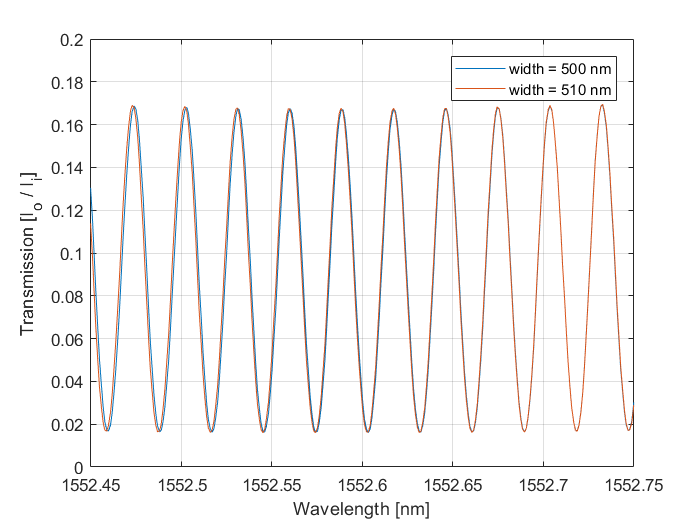
\includegraphics[width = 3.25in]{fig/michaelson_in-phase.png}
  \caption{Transfer function of two Michelson interferometers with different width, zoomed in on a region where the transfer functions are nearly in phase.}
  \label{fig:mich-in}
\end{figure}

\begin{figure}[t!]
  \centering
  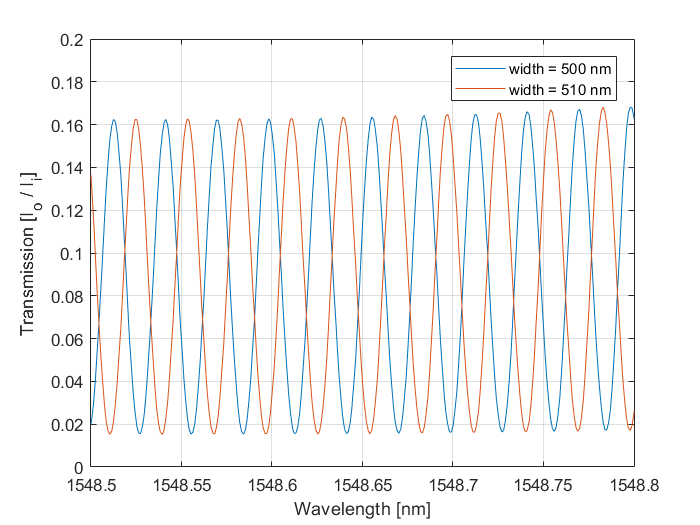
\includegraphics[width = 3.25in]{fig/michaelson_out-of-phase.png}
  \caption{Transfer function of two Michelson interferometer with different width, zoomed in on a region where the transfer functions are approximately $\pi$ shifted from each other.}
  \label{fig:mich-out}
\end{figure}

As a sanity check that this analysis should work, we can calculate the difference in FSR between these two data sets and plug this into equation \ref{eq:dw}. Before we can do this, we need to compute a value of $\frac{dn_g}{dw}$. This can be done by simulating $n_g$ near 1550nm for a few different waveguide widths in Lumerical MODE, and performing a linear fit on the resulting data, as shown in figure \ref{fig:dngdw}, which gives a value of $-1.691 \times 10^{-3} \text{nm}^{-1}$. From this, we can calculate a difference in width $\Delta w = 9.6$ nm on a pair of simulations that had a difference in width of 10 nm.

\begin{figure}[t!]
  \centering
  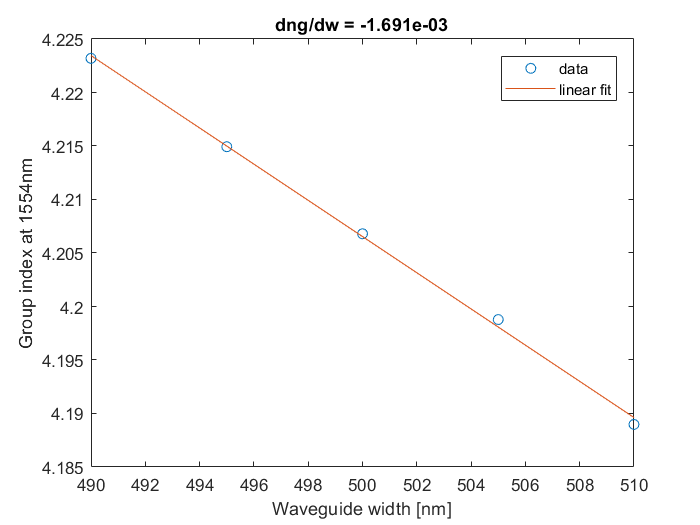
\includegraphics[width = 3.25in]{fig/dngdw.png}
  \caption{Variation in group index of the waveguide as a function of the waveguide width}
  \label{fig:dngdw}
\end{figure}

Finally, we show the proposed layout for all the devices on this chip in figure \ref{fig:layout}. This design was built using the SiEPIC PDK and is compact enough to fit into an area of $605 \mu m \times 410 \mu m $.

\begin{figure}[t!]
  \centering
  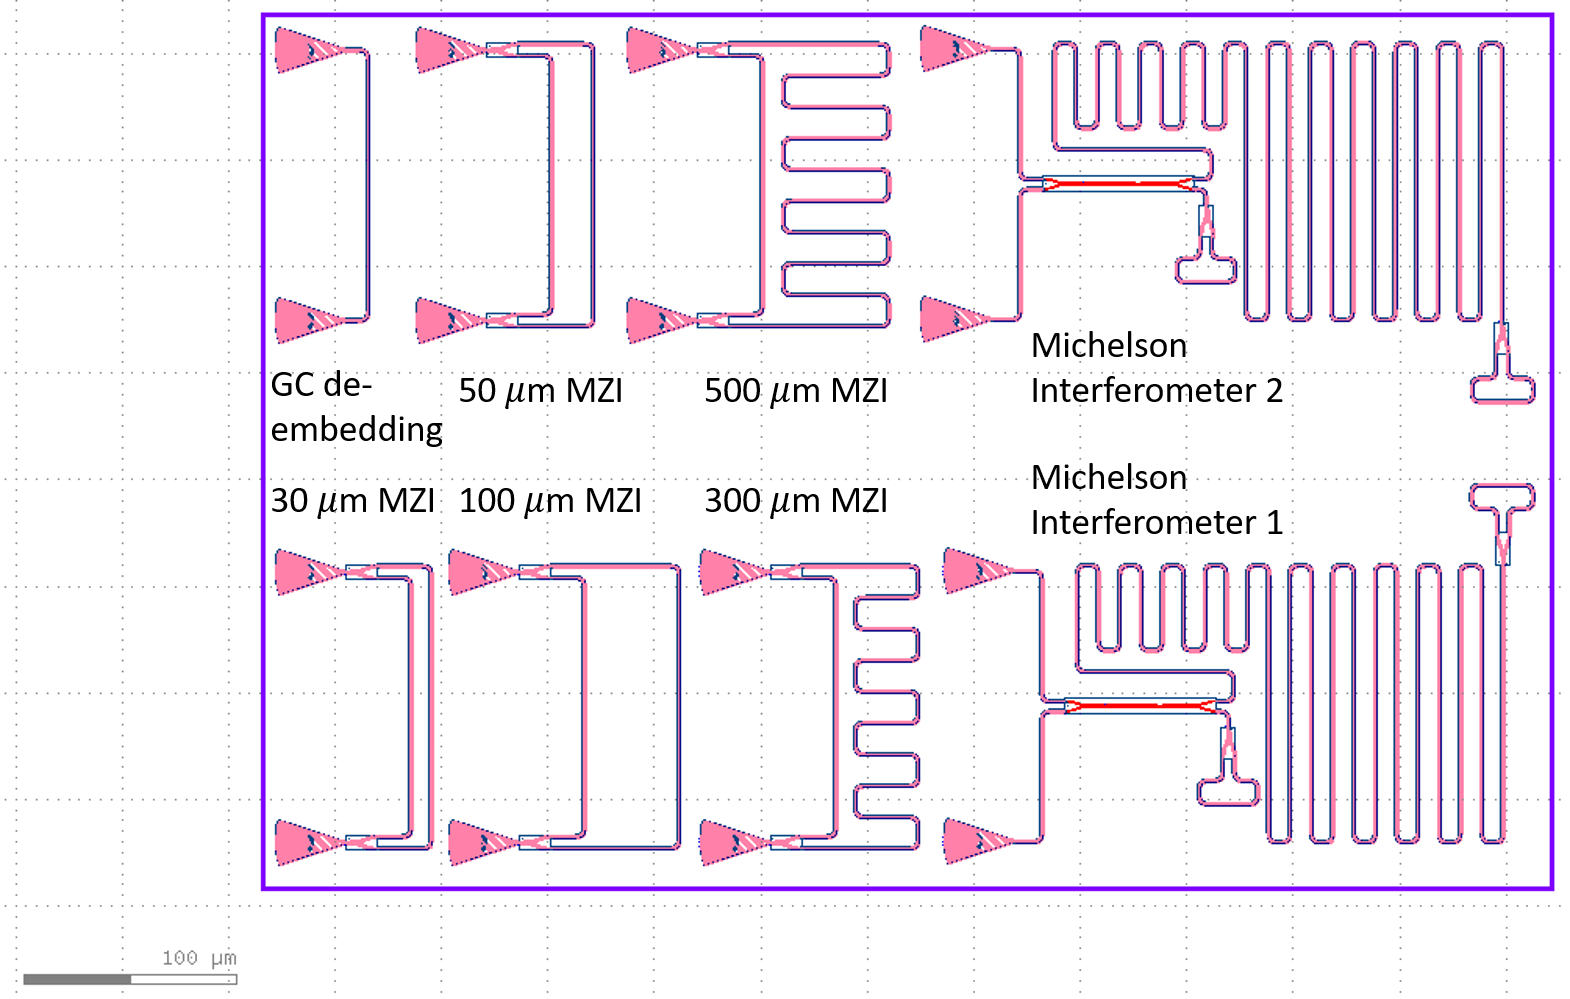
\includegraphics[width = 3.25in]{fig/layout.png}
  \caption{Layout for the proposed design, including the five Mach-Zehnder interferometers labelled by their length imbalance, the two Michelson interferometers, and a pair of grating couplers connected by a single waveguide to calibrate out the effects of the grating couplers.}
  \label{fig:layout}
\end{figure}

\section{Fabrication variability analysis}

The above simulations were computed assuming an ideal waveguide that is 500 nm wide and 220 nm thick. In reality, we expect there to be variations from device to device due to imperfections in the thickness of the Si layer in the SOI wafer as well as imperfections in the fabrication of the waveguide. A corner analysis of the expected variations in waveguide properties as well as device characteristics given an up to 1 standard deviation variation in these parameters is shown in table \ref{tab:corner}. Note that the values of $n_{\text{eff}}$ and $n_g$ were computed through FDTD simulation using the specified width and  thickness, and the FSR was calculated for a simulated MZI with a length imbalance of 100 $\mu m$ using the resulting compact model of the waveguide.

\begin{table}
\centering
\begin{tabular}{ r | r | r | r }
  \hline
  width, thickness [nm] & $n_{\text{eff}}$ & $n_g$ & FSR [nm] \\
  \hline
  (nominal) 500, 220.0  & 2.442            & 4.177 & 5.753  \\
  470, 215.3            & 2.371            & 4.229 & 5.680  \\
  470, 223.1            & 2.399            & 4.237 & 5.665  \\
  510, 215.3            & 2.439            & 4.159 & 5.773  \\
  510, 223.1            & 2.466            & 4.166 & 5.770  \\
\end{tabular}
\caption{Corner analysis of the effective index, group index, and free spectral range of an MZI with a length imbalance of 100 $\mu m$. The variations in thickness are a ``worst case scenario" variation, using the the specified 1 standard deviation variability in the Si layer thickness in the SOI wafer from Soitec. The width range is an estimate of the variability in waveguide thickness form past fabrication runs at the SiEPIC foundry.}
\label{tab:corner}
\end{table}

\section{Final device performance}

TODO

\section{Fabrication and measurement}
% 
% The waveguides used in this device will be fabricated on SOI wafer with a 220nm layer of Si on a buried oxide (BOX), and the waveguides will be fabricated to be 500 nm wide, with light coupled in via the quasi-TE mode of the waveguide. A finite-difference time domain (FDTD) simulation of this structure (shown in cross section, with an additional oxide capping layer) is shown in figure \ref{fig:mode}, with the spatial extent of the amplitude of the TE mode also shown.

The photonic devices were fabricated using the NanoSOI MPW fabrication process by Applied Nanotools~\cite{ANT} which is based on direct-write 100 keV electron beam lithography technology. Silicon-on-insulator wafers of 200 mm diameter, 220 nm device thickness and 2 $\mu$m buffer oxide thickness are used as the base material for the fabrication. The wafer was pre-diced into square substrates with dimensions of 25x25 mm, and lines were scribed into the substrate backsides to facilitate easy separation into smaller chips once fabrication was complete. After an initial wafer clean using piranha solution (3:1 H$_2$SO$_4$:H$_2$O$_2$) for 15 minutes and water/IPA rinse, hydrogen silsesquioxane (HSQ) resist was spin-coated onto the substrate and heated to evaporate the solvent. The photonic devices were patterned using a Raith EBPG 5000+ electron beam instrument using a raster step size of 5 nm. The exposure dosage of the design was corrected for proximity effects that result from the backscatter of electrons from exposure of nearby features. Shape writing order was optimized for efficient patterning and minimal beam drift. After the e-beam exposure and subsequent development with a tetramethylammonium sulfate (TMAH) solution, the devices were inspected optically for residues and/or defects. The chips were then mounted on a 4” handle wafer and underwent an anisotropic ICP-RIE etch process using chlorine after qualification of the etch rate. The resist was removed from the surface of the devices using a 10:1 buffer oxide wet etch, and the devices were inspected using a scanning electron microscope (SEM) to verify patterning and etch quality. A 2.2 $\mu$m oxide cladding was deposited using a plasma-enhanced chemical vapour deposition (PECVD) process based on tetraethyl orthosilicate (TEOS) at 300$^{\text{o}}$C. Reflectrometry measurements were performed throughout the process to verify the device layer, buffer oxide and cladding thicknesses before delivery.

To characterize the devices, a custom-built automated test setup~\cite{Chrostowski2015, MLP} with automated control software written in Python was used~\cite{siepic}.  An Agilent 81600B tunable laser was used as the input source and Agilent 81635A optical power sensors as the output detectors. The wavelength was swept from 1500 to 1600 nm in 10 pm steps.  A polarization maintaining (PM) fiber array was used to couple light in/out of the chip~\cite{PLC}. This maintained the polarization state of the light to couple the TE polarization into the grating couplers~\cite{Wang2014}.


\section*{Acknowledgments}

I acknowledge the edX UBCx Phot1x Silicon Photonics Design, Fabrication and Data Analysis course, which is supported by the Natural Sciences and Engineering Research Council of Canada (NSERC) Silicon Electronic-Photonic Integrated Circuits (SiEPIC) Program. The devices were fabricated by Cameron Horvath at Applied Nanotools, Inc. Hossam Shoman performed the measurements at The University of British Columbia. I acknowledge Lumerical Solutions, Inc., Mathworks, Mentor Graphics, Python, and KLayout for the design software.



% \clearpage

\bibliographystyle{ieeetr}
\bibliography{library}

\end{document}